% Tento soubor nahraďte vlastním souborem s přílohami (nadpisy níže jsou pouze pro příklad)
% This file should be replaced with your file with an appendices (headings below are examples only)

% Umístění obsahu paměťového média do příloh je vhodné konzultovat s vedoucím
% Placing of table of contents of the memory media here should be consulted with a supervisor
\chapter{Obsah přiloženého paměťového média}
\begin{itemize}
\item \texttt{README.TXT} -- Obsahuje informace o aplikaci a její instalaci
\item \texttt{BUILD\_MANUAL.TXT} -- Návod k překladu projektu
\item \texttt{doc/}
    \begin{itemize}
        \item \texttt{thesis/} -- Text této práce a zdrojové kódy \LaTeX
        \item \texttt{doxygen/} -- Dokumentace zdrojového kódu C++
        \item \texttt{javadoc/} -- Dokumentace zdrojového kódu Java
    \end{itemize}
\item \texttt{poster/} -- Plakát
\item \texttt{video/} -- Demonstrační video
\item \texttt{src/} -- Zdrojové kódy projektu
\item \texttt{utils/} -- Pomocný program
\item \texttt{config/} -- Dodatečné soubory nutné k běhu projektu
\end{itemize}

%\chapter{Manuál}

%\chapter{Konfigurační soubor} % Configuration file

%\chapter{RelaxNG Schéma konfiguračního souboru} % Scheme of RelaxNG configuration file

\chapter{Diagramy tříd}\label{app:class_diag}
\begin{figure}[H]\label{app:voice_activity_detection}
	\centering
		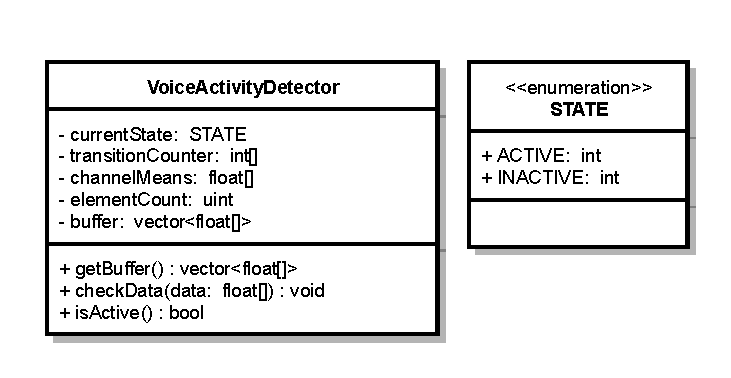
\includegraphics[height=5cm]{obrazky-figures/classdiagram_voiceactivitydetection.pdf}
        \caption{Diagram tříd detekce řečové aktivity}
\end{figure}
\begin{figure}[H]\label{app:feature_extraction}
	\centering
		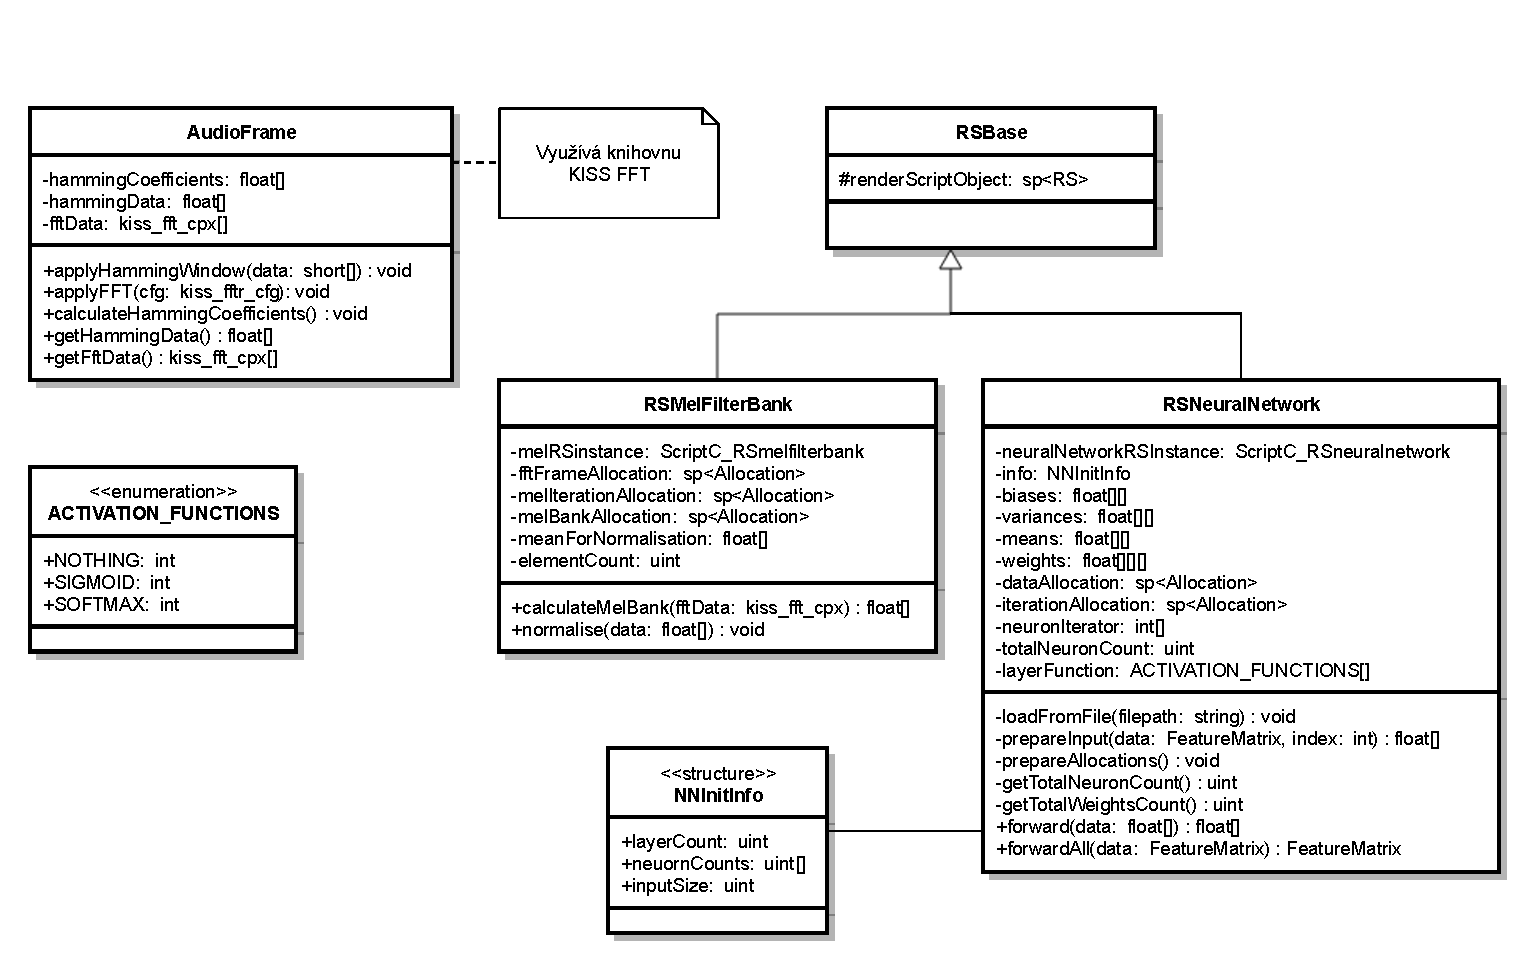
\includegraphics[height=14cm, angle=90]{obrazky-figures/classdiagram_featureextraction.pdf}
        \caption{Diagram tříd extrakce příznaků}
\end{figure}
\begin{figure}[H]\label{app:decoder}
	\centering
		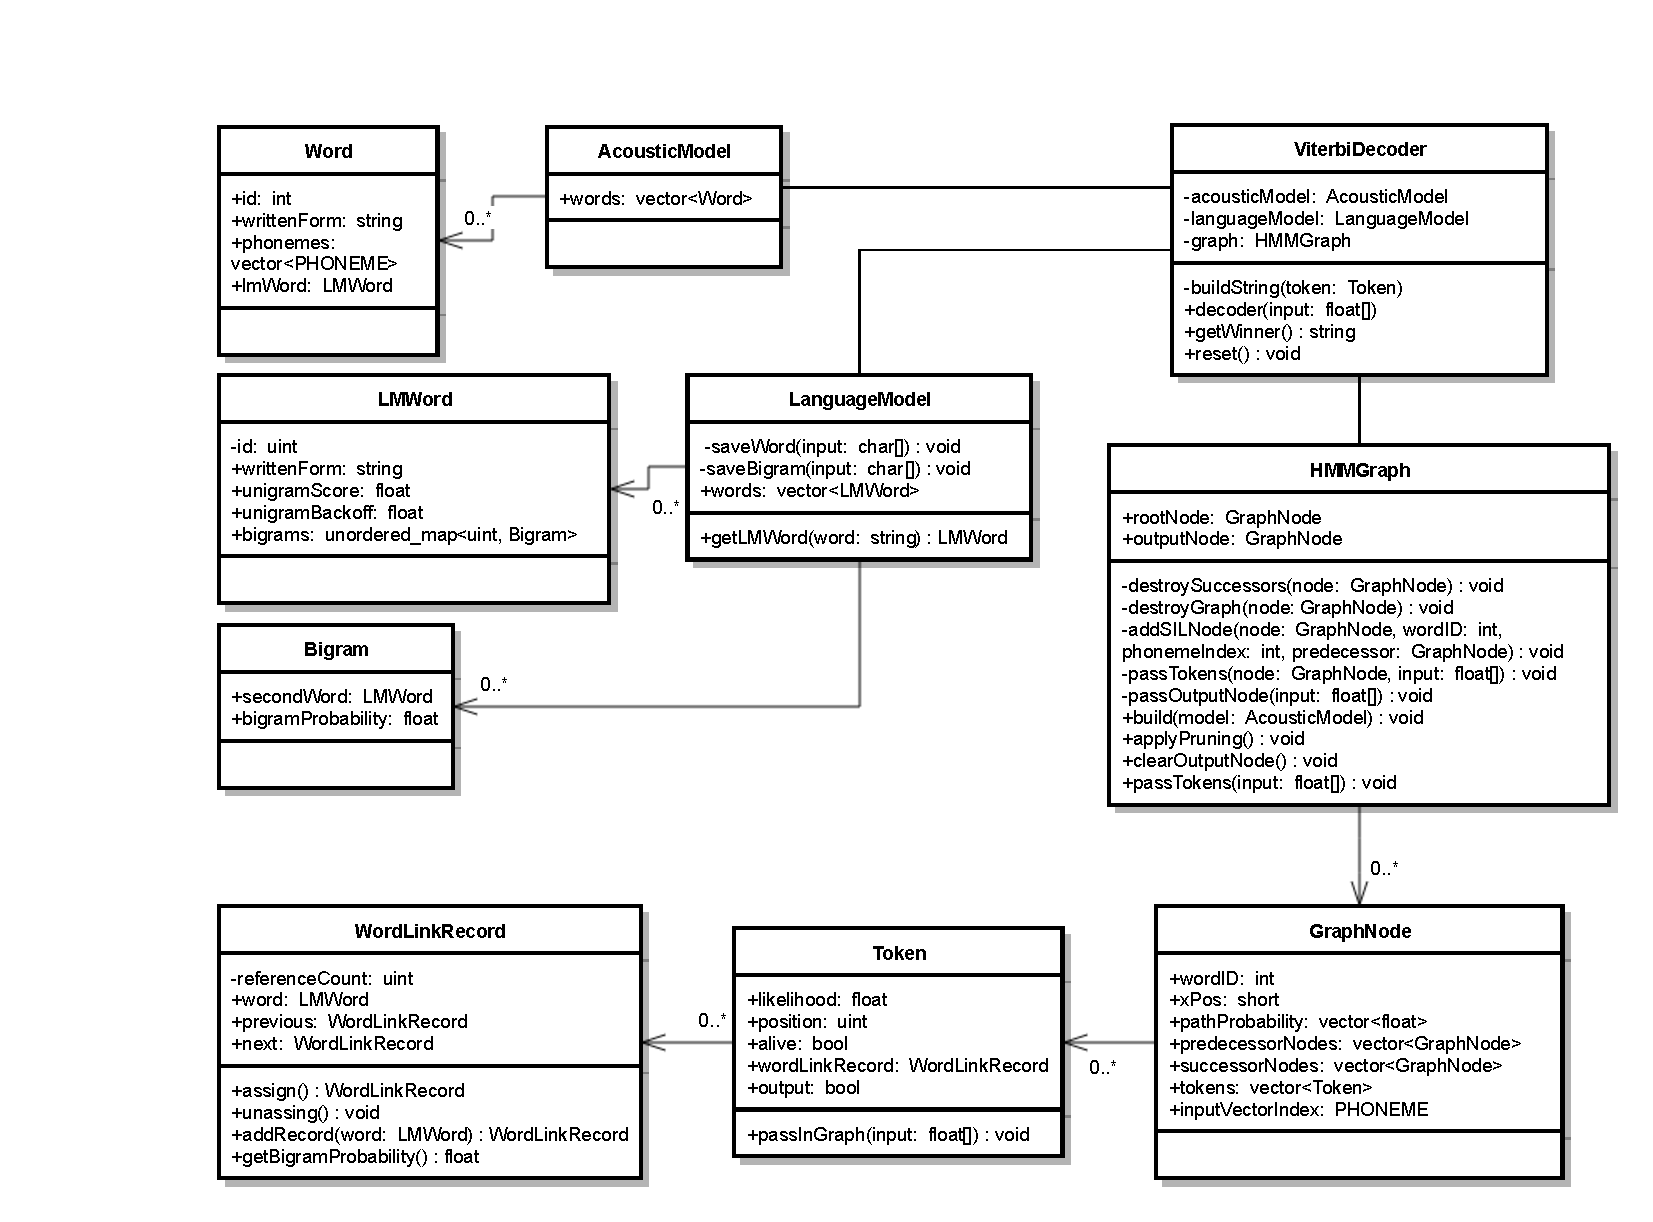
\includegraphics[height=16cm, angle=90]{obrazky-figures/classdiagram_decoder.pdf}
        \caption{Diagram tříd dekodéru}
\end{figure}
\begin{figure}\label{app:threads}
	\centering
		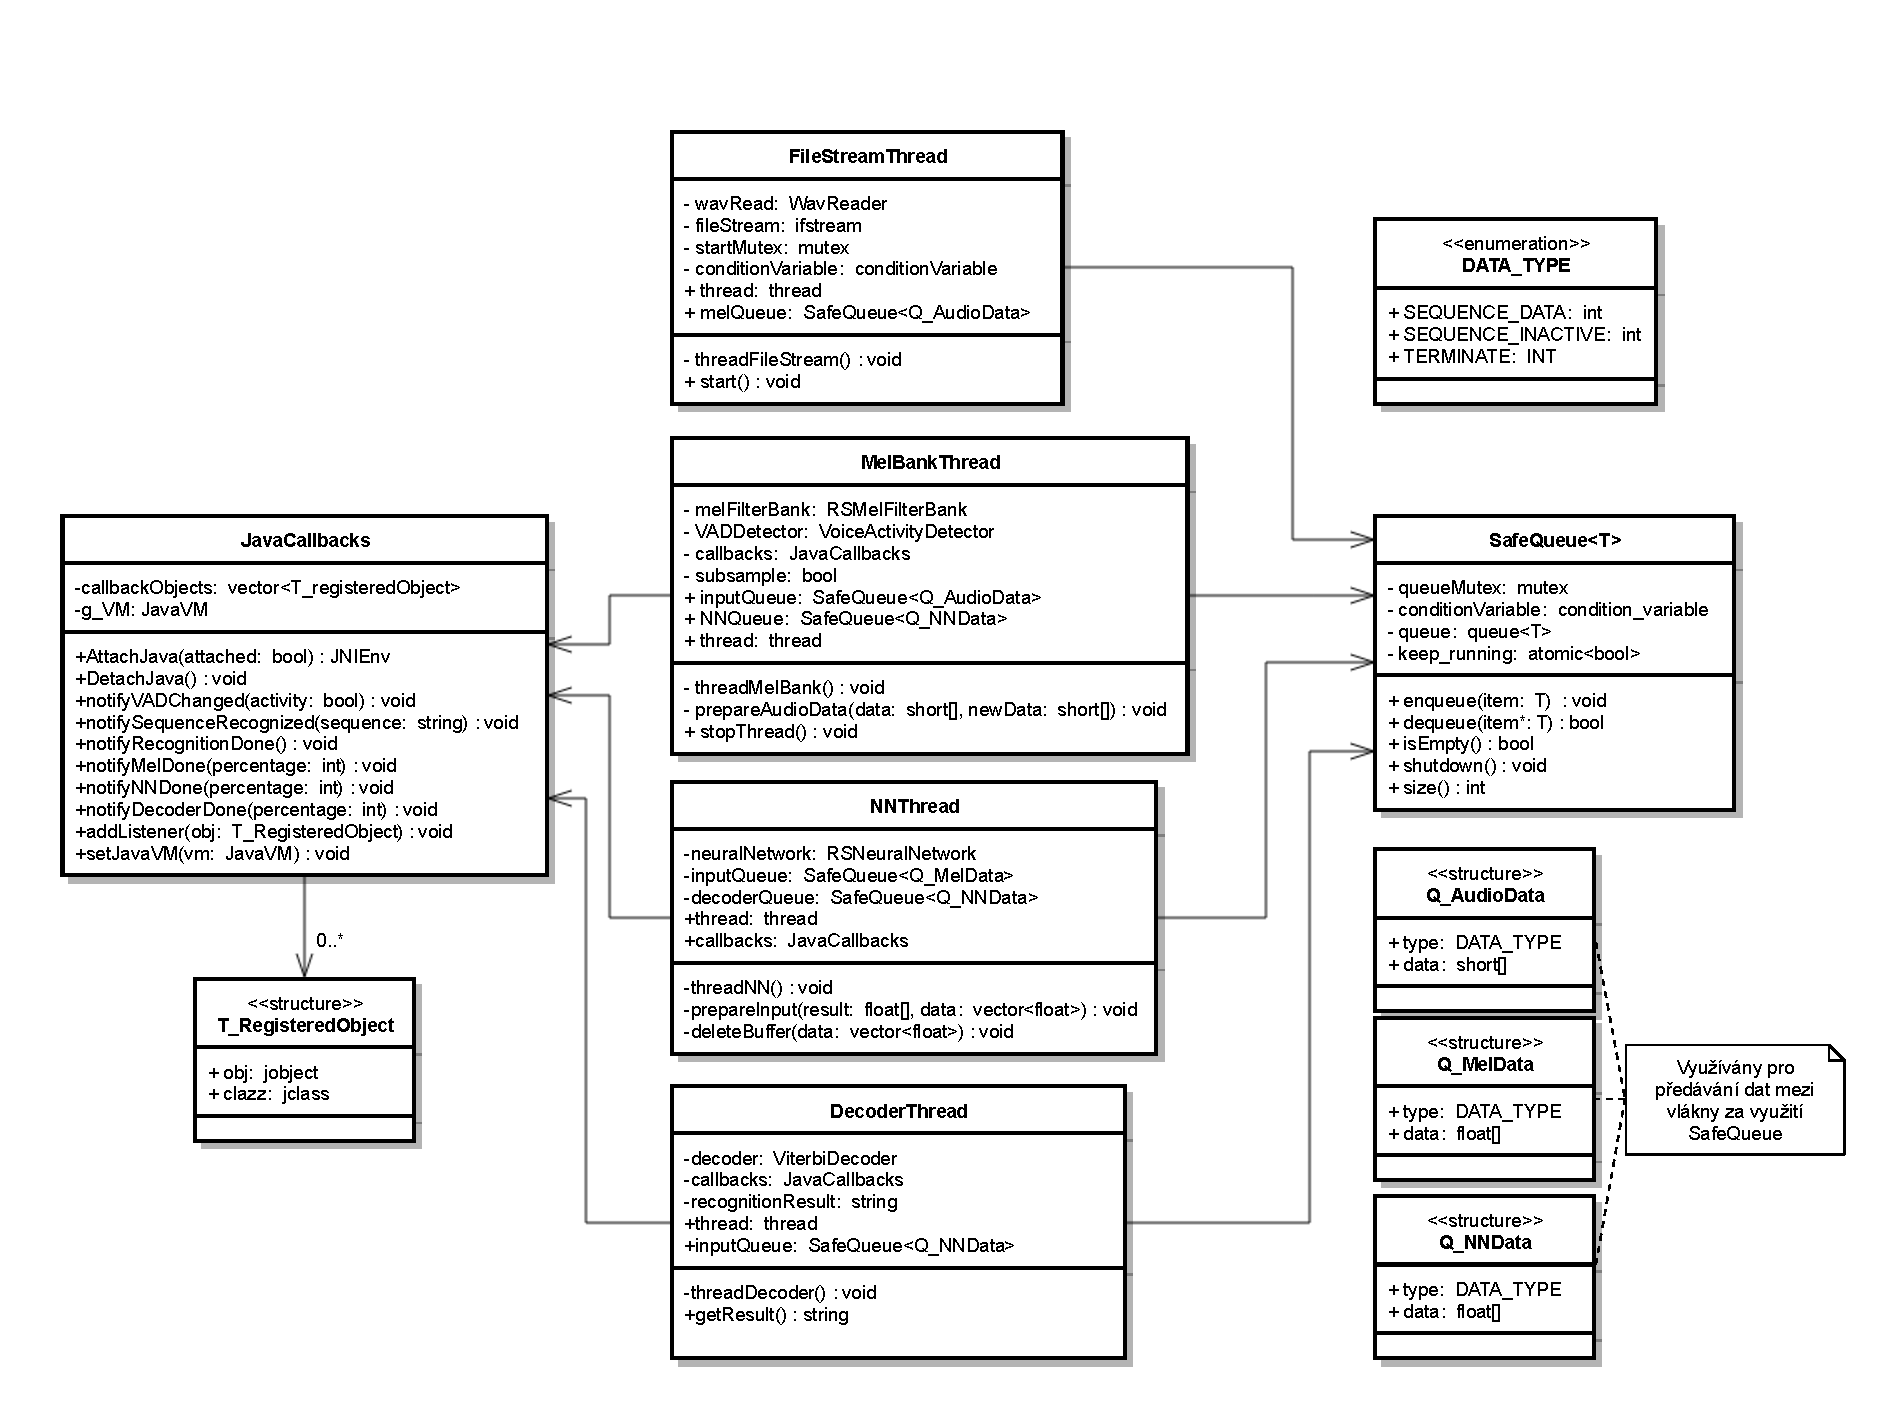
\includegraphics[height=16cm, angle=90]{obrazky-figures/classdiagram_threads.pdf}
        \caption{Diagram tříd vláken}
\end{figure}
\begin{figure}[H]\label{app:utility}
	\centering
		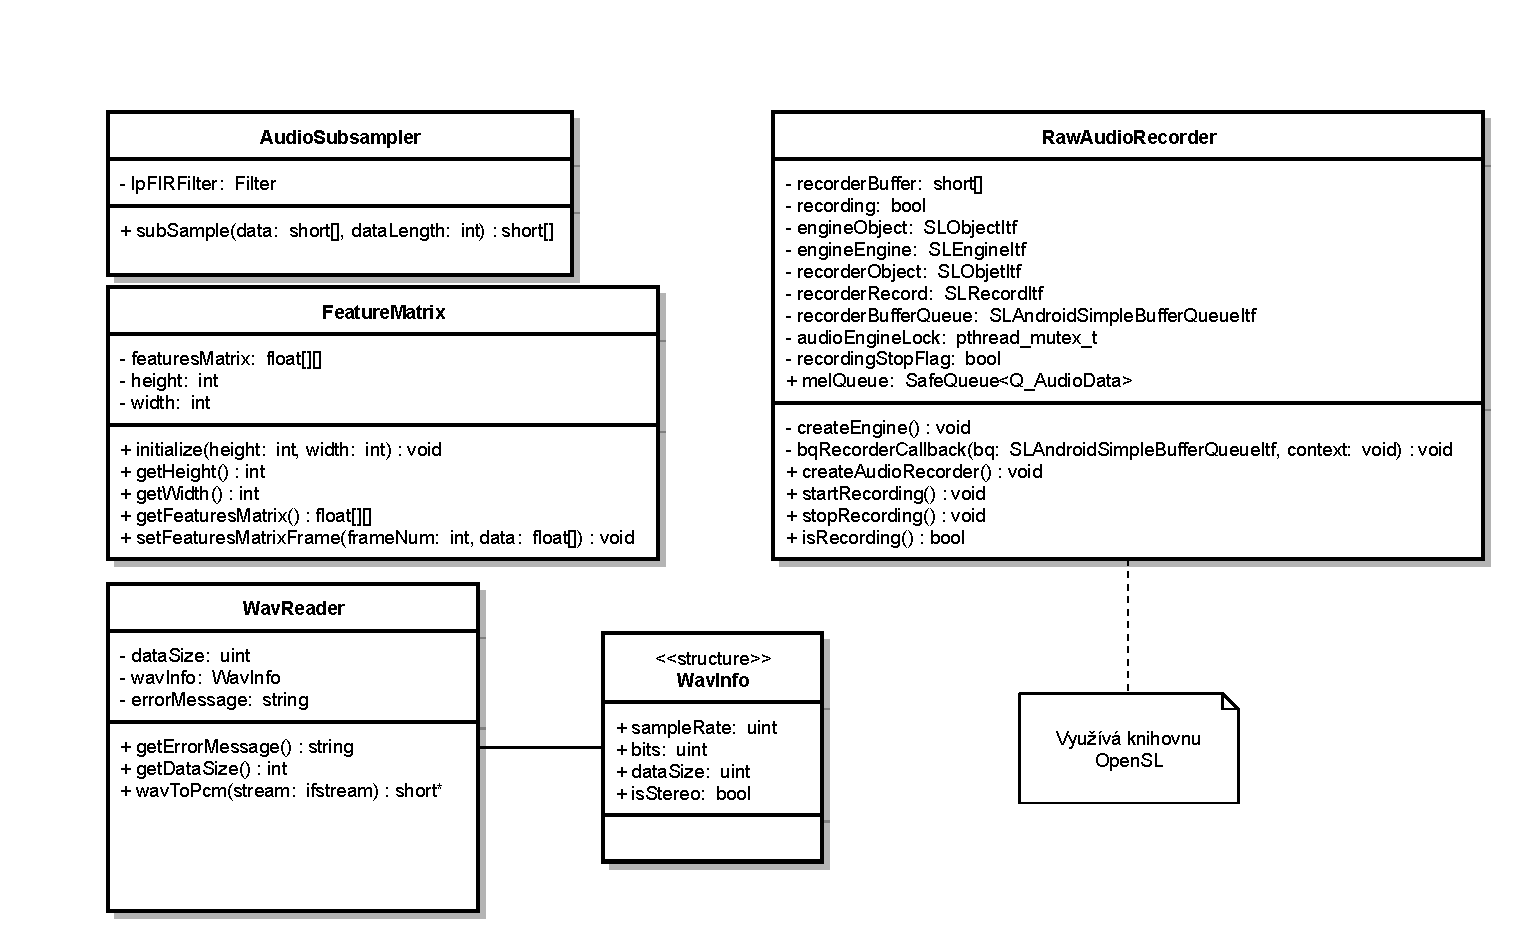
\includegraphics[height=14cm, angle=90]{obrazky-figures/classdiagram_utility.pdf}
        \caption{Diagram pomocných tříd}
\end{figure}